\label{chapter:applications}

In this chapter we discuss applications of our improvements to the binary XPFC model.
To begin we'll discuss an effective equation of motion in the limit that density 
change on solidification is small, after which we'll examine the to process of
multi-step nucleation of nanoparticles from solution. To conclude we'll discuss
areas of future application.

%%%%%%%%%%%%%%%%%%%%%%%%%%%%%%%%%%%%%%%%%%%%%%%%%%%%%
\subsection{Dynamics in the small $\Delta n$ limit} %
%%%%%%%%%%%%%%%%%%%%%%%%%%%%%%%%%%%%%%%%%%%%%%%%%%%%%

{
    \color{ForestGreen} Develop the dynamics from DDFT and show (with references
    to the relevant papers that these dynamics are valid in the small density
    change limit specifically
}

%%%%%%%%%%%%%%%%%%%%%%%%%%%%%%%%%%%%%%%%%%%%%%%%%%%%%%%%%%%%%
\section{Multistep Nucleation of Nanoparticles in Solution} %
%%%%%%%%%%%%%%%%%%%%%%%%%%%%%%%%%%%%%%%%%%%%%%%%%%%%%%%%%%%%%

{
    \color{ForestGreen} Discuss the interest in this process with reference to 
    papers about multistep nucleation theories. Discuss relevance of nanoparticles
    size and prediction of size (catalyzsis, color, etc... size is the basic relevant
    detail of nanoparticles).
}

\begin{figure}
    \centering
    \begin{subfigure}[b]{0.3\textwidth}
        
\includegraphics[width=\textwidth]{initial}
        \label{fig:initial}
        \caption{}
    \end{subfigure}
    ~
    \begin{subfigure}[b]{0.3\textwidth}
        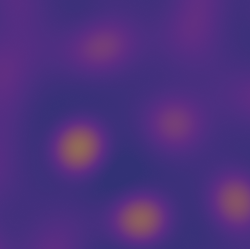
\includegraphics[width=\textwidth]{early_spinodal}
        \label{fig:early_spinodal}
        \caption{}
    \end{subfigure}
    ~
    \begin{subfigure}[b]{0.3\textwidth}
        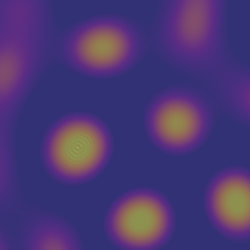
\includegraphics[width=\textwidth]{devel_spinodal.png}
        \label{fig:devel_spinodal}
        \caption{}
    \end{subfigure}

    \vspace{0.5cm}
    \begin{subfigure}[b]{0.3\textwidth}
        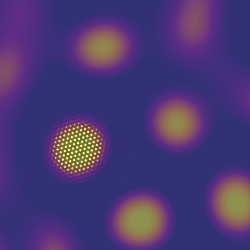
\includegraphics[width=\textwidth]{nucleation}
        \label{fig:nucleation}
        \caption{}
    \end{subfigure}
    ~
    \begin{subfigure}[b]{0.3\textwidth}
        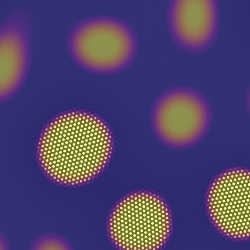
\includegraphics[width=\textwidth]{nucleation_and_sacrificial_growth}
        \label{fig:nucleation_and_growth}
        \caption{} 
    \end{subfigure}
    ~
    \begin{subfigure}[b]{0.3\textwidth}
        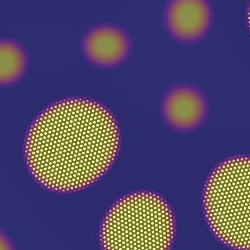
\includegraphics[width=\textwidth]{sacrificalgrowth}
        \label{fig:sacrifical_growth}
        \caption{}
    \end{subfigure}
    
    \vspace{0.5cm}
    \begin{subfigure}[b]{0.3\textwidth}
        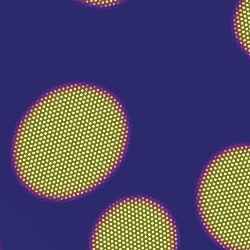
\includegraphics[width=\textwidth]{crystalgrowth}
        \label{fig:crystalgrowth}
        \caption{}
    \end{subfigure}
    ~
    \begin{subfigure}[b]{0.3\textwidth}
        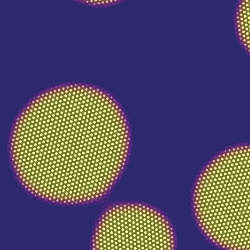
\includegraphics[width=\textwidth]{crystalgrowth2}
        \label{fig:crystalgrowth2}
        \caption{}
    \end{subfigure}
    ~ 
    \begin{subfigure}[b]{0.3\textwidth}
        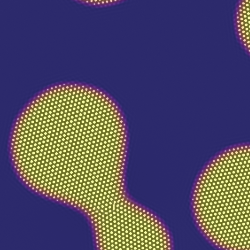
\includegraphics[width=\textwidth]{crystalgrowth3}
        \label{fig:crystalgrowth3}
        \caption{}
    \end{subfigure}
    \label{fig:preciptiation}
    \caption{Precipitation of nanoparticles from solution}
\end{figure}


%%%%%%%%%%%%%%%%%%%%%%%%%%%%%%%
\section{Future Applications} %
%%%%%%%%%%%%%%%%%%%%%%%%%%%%%%%

